
\chapter{Pilot-Proxy Estimation: Statistics, Transfer, \& Validation}
\label{sec:estimator}
\label{sec:pipeline}

This chapter follows the evidence ladder of Section~\ref{sec:system:detector}: mathematical definition, known-input tests, offline archive transfer, and online shadow evaluation. Estimation remains threshold-free throughout. It produces a pilot-inferred shelf-SNR coordinate; Chapter~\ref{sec:detection} decides whether that estimate and the fine statistic warrant a mask.

\section{Mathematical Estimator}

\subsection{Problem Formulation \& System Definitions}
\label{sec:pipeline:problem}

Consider a multichannel receiving array consisting of $M = 2048$ spatial feeds operating over a discrete time frame of $N = 16384$ complex baseband samples. Let the received data frame be represented by the matrix $\mathbf{X} \in \mathbb{C}^{M \times N}$, where the scalar element $x_{m,n}$ denotes the sample acquired from feed $m \in \{0, 1, \dots, M-1\}$ at sample index $n \in \{0, 1, \dots, N-1\}$:
\begin{equation}
\mathbf{X} = \begin{bmatrix}
x_{0,0} & x_{0,1} & \dots & x_{0, N-1} \\
x_{1,0} & x_{1,1} & \dots & x_{1, N-1} \\
\vdots & \vdots & \ddots & \vdots \\
x_{M-1,0} & x_{M-1,1} & \dots & x_{M-1, N-1}
\end{bmatrix}.
\end{equation}
The objective of the estimation chain is to measure, once per frame, the excess power of a narrow pilot-like component relative to its local background. Chapter~\ref{sec:detection} turns that measured statistic into a binary decision. In the analytical model,
\begin{align}
H_0: &\quad x_{m,n}=n_{m,n}, \\
H_1: &\quad x_{m,n}=a_m e^{j(2\pi \nu n+\phi_m)}+n_{m,n},
\end{align}
where $a_m$ and $\phi_m$ are feed-dependent nuisance parameters, $\nu$ lies in the fine search window around the synthesized pilot frequency, and $n_{m,n}$ is initially modeled as circular complex Gaussian noise.  This is the model under which the tone projection has the matched-filter interpretation; local references, rank normalization, frequency search, quantization, feed covariance, and empirical calibration are additional parts of the complete detector and are not covered by that simple optimality statement.

The background power is unknown and time-varying --- receiver gain, sky temperature, and broadband interference all modulate it --- so the test must be invariant to the absolute noise scale. This requirement shapes the entire pipeline: every statistic below is ultimately a \emph{ratio} of target-matched power to reference-matched power.  Under the idealized $H_0$ model the common scale $\sigma^2$ cancels.  In operation, the thresholds are calibrated empirically rather than assumed to transfer perfectly across gain states; the ratio construction removes first-order scale dependence, while the measured null retains receiver correlations and non-Gaussian structure.

\begin{figure}[t]
\centering
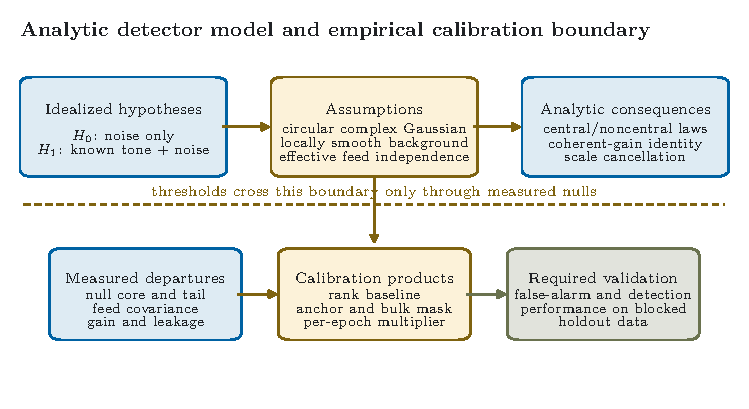
\includegraphics[width=0.98\linewidth]{figs/fig_model_calibration_layers.pdf}
\caption[Analytical model and empirical calibration layers]{The detector has two evidence layers.  The upper layer is the analytical known-tone, circular-Gaussian model used to derive the projection and idealized null.  The lower layer contains the instrument-specific effects that set the actual operating point: the measured null core and tails, feed covariance, gain and leakage, and per-epoch null calibration.  A theorem about the upper layer does not by itself establish global optimality of the complete lower-layer decision.}
\label{fig:pipeline:modelcal}
\end{figure}

The test signal is defined by a length-$K$ weight profile against background noise estimated from auxiliary reference profiles. The weight coefficient vector length is fixed at $K = 128$ taps. We define $R = 3$ distinct weight profiles: one target profile ($r = 0$) and $N_{\text{ref}} = 2$ reference profiles ($r \in \{1, 2\}$). The reference profiles are the target profile displaced by $\pm 2$ bins of the length-$K$ filter's spectral grid (distinct from the fine bins of Section~\ref{sec:pipeline:coherent}), leaving a one-bin guard separation between target and reference, thereby establishing a spectrally local background estimate; their construction and the justification of every dimension are given in Chapter~\ref{sec:param}. These profiles are assembled into the weight matrix $\mathbf{W} \in \mathbb{C}^{K \times R}$:
\begin{equation}
\mathbf{W} = \begin{bmatrix}
\mathbf{w}_{\text{target}} & \mathbf{w}_{\text{ref,1}} & \mathbf{w}_{\text{ref,2}}
\end{bmatrix}.
\end{equation}
\textit{Remark on fixed-point arithmetic:} In the physical architecture, input samples and weight coefficients are packed as complex integer \texttt{int4} values with exact integer accumulation and frozen fixed-point FFT arithmetic that is bit-identical between reference software and GPU execution. While this section formulates the pipeline using continuous complex variables for analytical clarity, complete quantization and fixed-point implementation details are deferred to Chapter~\ref{sec:impl}. The formulation is nonetheless exact in structure: every sum written below is computed as written, in integer arithmetic, with accumulator widths chosen in Section~\ref{sec:param:tradeoffs} so that no rounding or saturation occurs in the projections or coarse power sums before the final ratio; the one specified departure from real arithmetic is the frozen rounding inside the fine-axis transform of Section~\ref{sec:impl:fxfft}, and ``exact'' throughout means bit equality with that specification, not equivalence to floating point. Figure~\ref{fig:pipeline} summarizes the estimator and previews the policy boundary developed in Chapter~\ref{sec:detection}.

\begin{figure}[t]
\centering
\resizebox{\linewidth}{!}{% Editable source for Figure \ref{fig:pipeline}: the processing chain as a DSP block diagram.
\begin{tikzpicture}[font=\small, x=1cm, y=1cm,
  b/.style={blk, text width=26mm, minimum height=10mm}, bm/.style={blkm, text width=26mm, minimum height=10mm},
  bc/.style={blkc, text width=26mm, minimum height=10mm}, bx/.style={blkx, text width=26mm, minimum height=10mm}]
% ---------------- row 1: projection
\node[b] (x) at (-0.4,0) {$x_m[n]$: $M$ inputs, \texttt{int4}};
\node[b] (seg) at (3.5,0) {segment into $L$ windows of $K$};
\node[op] (mul) at (6.1,0) {$\times$};
\node[bm, text width=30mm] (w) at (6.6,1.45) {profiles $w_r[k]$: target and two references};
\pic at (4.45,1.45) {impulse};
\node[op] (sumk) at (7.4,0) {$\sum_k$};
\node[b] (z) at (10.0,0) {$Z_m[\ell,r]$: exact row sums, one per window and profile};
\draw[bus] (x) -- (seg) node[width, pos=0.5, above, yshift=1pt]{$4{+}4$ b};
\draw[sig] (seg) -- (mul); \draw[sigm] (w.south -| mul) -- (mul);
\draw[sig] (mul) -- (sumk); \draw[sig] (sumk) -- (z) node[width, midway, above]{int32};
% ---------------- row 2: fine spectra
\node[b] (pad) at (3.5,-2.5) {zero-pad $L \to L_F = 256$};
\node[b, text width=20mm] (fft) at (6.4,-2.5) {DFT across the windows};
\pic at (6.15,-3.32) {butterfly};
\node[op] (sq) at (9.0,-2.5) {$|\cdot|^2$};
\node[op] (summ) at (10.2,-2.5) {$\sum_m$};
\node[b] (s) at (12.7,-2.5) {$S_r[f]$: \texttt{uint64} fine powers, $3\times256$};
\draw[sig] (z.south) -- ++(0,-0.8) -| (pad.north);
\draw[sig] (pad) -- (fft); \draw[sig] (fft) -- (sq) node[width, pos=0.4, above]{Q15}; \draw[sig] (sq) -- (summ);
\draw[sig] (summ) -- (s) node[width, midway, above]{64 b};
% ---------------- row 3: fine decision
\node[op] (rat) at (12.7,-4.6) {$\div$};
\node[b, text width=22mm] (mx) at (9.4,-4.2) {$\max_{\mathcal D} T[f]$ (designated window)};
\node[bm, text width=22mm] (rank) at (9.4,-5.7) {rank select $T_{(\rho)}$ over the bulk $\mathcal B$};
\node[opm] (eta) at (7.4,-5.7) {$\times\eta$};
\node[cmp, shape border rotate=180, minimum height=10mm] (c1) at (5.8,-4.95) {$>$};
\node[bc] (mask) at (3.2,-4.95) {mask bit $+$ validity, one per frame};
\draw[sig] (s) -- (rat);
\node[width, anchor=west] at (12.3,-5.4) {$T[f]=\frac{2S_0[f]}{S_1[f]+S_2[f]}$};
\draw[sig] (rat.west) -- ++(-0.6,0) |- (mx.east);
\draw[sig] (rat.west) -- ++(-0.6,0) |- (rank.east);
\draw[sig] (mx.west) -- ++(-0.35,0) |- ([yshift=1.7mm]c1.east);
\draw[sigm] (rank) -- (eta); \draw[sigm] (eta.west) -- ++(-0.35,0) |- ([yshift=-1.7mm]c1.east);
\draw[sigc] (c1) -- (mask);
\node[lab, text width=46mm] at (9.4,-6.75) {bundle data per channel and era: $(f_a,\mathcal D,\mathcal B,\rho,\eta_{q16})$};
% ---------------- row 4: coarse marginal
\node[op] (sq2) at (1.5,-8.3) {$|\cdot|^2$};
\node[op] (sum2) at (2.8,-8.3) {$\sum_{m,\ell}$};
\node[b, text width=20mm] (p) at (4.9,-8.3) {$P_r$: \texttt{uint64} coarse marginals};
\node[op] (rat2) at (7.0,-8.3) {$\div$};
\node[cmp, minimum height=9mm] (c2) at (9.0,-8.3) {$F>\mu_0$};
\node[bx] (flag) at (11.9,-8.3) {survey flag $F>\mu_0$: a per-frame mechanism check, recorded, never a decision};
\draw[sig] (z.south west) -- ++(0,-0.6) -- ++(-11.4,0) |- (sq2.west);
\draw[sig] (sq2) -- (sum2); \draw[sig] (sum2) -- (p);
\draw[sig] (p) -- (rat2);
\node[width] at (7.0,-9.25) {$F=\frac{2P_0}{P_1+P_2}$}; \draw[sigm] (rat2) -- (c2); \draw[sigm] (c2) -- (flag);
\draw[ctl] (p.north) -- ++(0,0.35) -- ++(11.2,0) |- (z.east);
\node[lab, rotate=90, anchor=south, text width=84mm, align=center] at (16.3,-4.6) {exact tripwire: register $P_r$ $=$ row-sum $P_r$; Parseval holds only to the rounding bound};
\end{tikzpicture}
}
\caption[The pilot-proxy processing chain]{The pilot-proxy processing chain. The estimator of this chapter ends at $P_r$, $S_r[f]$, and $T[f]$. The rank, multiplier, and mask are shown only to mark the policy boundary developed in Chapter~\ref{sec:detection}. All quantities upstream of the recorded diagnostics are exact integers. The coarse marginal $P_r$ also supplies the Parseval verification tripwire of Section~\ref{sec:impl:verify}.}
\label{fig:pipeline}
\end{figure}

\subsection{Sub-Frame Segmentation \& Weight Projection}
\label{sec:pipeline:segmentation}

To apply the weight profiles across the temporal frame, each feed's time series of length $N$ is partitioned into $L = N / K = 128$ non-overlapping sub-frames of length $K$. Let $\mathbf{s}_{m,\ell} \in \mathbb{C}^{K \times 1}$ denote the $\ell$-th sub-frame column vector of the $m$-th feed, where $\ell \in \{0, 1, \dots, L-1\}$:
\begin{equation}
\mathbf{s}_{m,\ell} = \begin{bmatrix}
x_{m, \, \ell K} & x_{m, \, \ell K + 1} & \dots & x_{m, \, \ell K + (K-1)}
\end{bmatrix}^T.
\end{equation}
Concatenating all sub-frames across all feeds yields the reshaped data matrix $\mathbf{Y} \in \mathbb{C}^{K \times P}$, where $P = M L = 262144$ represents the total number of sub-frames across the array:
\begin{equation}
\mathbf{Y} = \begin{bmatrix}
\mathbf{s}_{0,0} & \dots & \mathbf{s}_{0, L-1} & \big| & \mathbf{s}_{1,0} & \dots & \mathbf{s}_{1, L-1} & \big| & \dots & \big| & \mathbf{s}_{M-1,0} & \dots & \mathbf{s}_{M-1, L-1}
\end{bmatrix}.
\end{equation}
The segmentation is purely an indexing view --- the sub-frames tile the frame exactly ($KL = N$, Section~\ref{sec:param:tradeoffs}), so no samples are discarded, duplicated, or windowed, and the reshape involves no data movement in implementation. The temporal projection of the data frame onto the $R$ weight profiles is evaluated via the matrix inner product:
\begin{equation}
\mathbf{Z} = \mathbf{W}^H \mathbf{Y} \in \mathbb{C}^{R \times P},
\end{equation}
where $(\cdot)^H$ denotes the Hermitian (conjugate transpose) operator. Each column $p \in \{0, 1, \dots, P-1\}$ of $\mathbf{Z}$ contains the complex response of the target and reference profiles for a specific feed $m = \lfloor p / L \rfloor$ and temporal sub-frame index $\ell = p \bmod L$. This single product --- $P = 262144$ length-$K$ complex projections per $41.94$~ms frame, three profiles each --- is the pipeline's dominant arithmetic cost, and the stage the packed-integer kernel geometry of Section~\ref{sec:param:tradeoffs} is designed around. Everything downstream operates on the $3 \times 262144$ projected values rather than the $2048 \times 16384$ raw samples: the projection is also a ${\sim}43\times$ reduction in value count (${\sim}11\times$ in bytes at the widened integer precision) that renders the remaining stages computationally minor.

\subsection{Coherent Spectral Integration}
\label{sec:pipeline:coherent}

The projection of Section~\ref{sec:pipeline:segmentation} is coherent only \emph{within} each $K$-sample sub-frame. A first-generation reduction may stop there: square each projection and sum the powers over all sub-frames and feeds (the coarse statistic of Section~\ref{sec:pipeline:noncoherent}). Such a reduction, however, discards the phase relationship \emph{between} successive sub-frames, which for the signal of interest is deterministic rather than random. A frequency-stable pilot line at residual offset $\Delta\nu$ from the synthesized tone advances its phase by exactly $2\pi \Delta\nu K$ between consecutive sub-frames of the same feed: the $L$ successive projections of a feed rotate deterministically, and integrating them coherently before squaring recovers deflection that incoherent summation forfeits. The available gain is substantial: coherent integration of $L$ sub-frames improves the deflection signal-to-noise ratio by up to $10 \log_{10} \sqrt{L} \approx 10.5$~dB over the incoherent baseline. Realizing it requires matching the unknown residual rotation --- which is precisely a spectral analysis across the sub-frame axis.

To exploit this temporal coherence, the projected matrix $\mathbf{Z}^T \in \mathbb{C}^{P \times R}$ is partitioned vertically into $M$ distinct feed blocks $\{\mathbf{B}_0, \mathbf{B}_1, \dots, \mathbf{B}_{M-1}\}$, where each block $\mathbf{B}_m \in \mathbb{C}^{L \times R}$ collects the $L$ sequential temporal projections for feed $m$, defining the triple-indexed entries $z_{m,\ell,r} \equiv z_{r, \, mL+\ell}$:
\begin{equation}
\mathbf{B}_m = \begin{bmatrix}
z_{m,0,0} & z_{m,0,1} & z_{m,0,2} \\
z_{m,1,0} & z_{m,1,1} & z_{m,1,2} \\
\vdots & \vdots & \vdots \\
z_{m,L-1,0} & z_{m,L-1,1} & z_{m,L-1,2}
\end{bmatrix}.
\end{equation}
Coherent temporal integration is performed by applying a zero-padded Discrete Fourier Transform (DFT) of length $L_F = 2L = 256$ independently across the sub-frame axis $\ell$ for each feed $m$ and weight profile $r$:
\begin{equation}
\widetilde{B}_m[f,r] = \sum_{\ell=0}^{L-1} B_m[\ell,r]\, e^{-j \frac{2\pi}{L_F} f \ell}, \qquad f \in \{0, 1, \dots, L_F-1\}.
\end{equation}
Each spectral bin $f$ coherently integrates the $L$ sub-frame projections under a frequency offset hypothesis of $f / (L_F K)$ cycles per sample (interpreted modulo the sub-frame rate: bins above $L_F/2$ correspond to negative offsets): the DFT evaluates all $L_F$ rotation hypotheses simultaneously, so no prior knowledge of the residual offset is needed --- the matched hypothesis corresponds to the bin of maximum response, whose index directly measures the pilot's residual frequency (the survey's per-channel \emph{anchor}, Section~\ref{sec:pipeline:decision}).

Two distinct scalloping mechanisms bound the recovered gain, and they are treated separately here. The first is the \emph{sub-frame projection rolloff}: the $K$-tap projection has the Dirichlet response of Eq.~\eqref{eq:dirichlet}, so a pilot at the edge of the fine span ($\pm f_s/2K$, i.e.\ half a coarse grid bin from the synthesized tone) is attenuated by $|D_K(1/2)| = 2/\pi$, a worst-case loss of $3.92$~dB. This loss is a property of the segmentation geometry, not of the transform; it is minimized in practice because the synthesized tone absorbs each channel's nominal offset exactly (Section~\ref{sec:param:target}), leaving typical residuals far inside the span. The second is \emph{fine-grid scalloping}: a residual falling between adjacent fine bins splits its energy. The zero-padding factor of 2 --- fine-bin spacing $(f_s/K)/L_F \approx 11.9$~Hz --- halves the worst-case bin-center mismatch; a further doubling would halve it again, but at double the transform cost and shared-memory footprint for a residual the decision stage already absorbs, so the factor-2 padding represents the practical optimum. What padding leaves is captured by the $\pm 2$-bin designated window of Section~\ref{sec:pipeline:decision}, and this width is not an additional free parameter: on the window axis, a residual tone's response is the $L$-point analogue of Eq.~\eqref{eq:dirichlet}, whose main lobe spans $\pm 1$ window-rate bin --- exactly $\pm 2$ bins of the padded grid. The designated window is therefore the kernel's \emph{main-lobe extent}: with the anchor measured to the nearest fine bin, the two dominant bins straddling any sub-bin residual always lie inside it.  Era-scale changes do not fit inside that guard: a station change can move the anchor by tens of fine bins and must create a new calibration epoch (Section~\ref{sec:tolerance:eras}). The two $\pm 2$ displacements in this architecture are thus dual applications of the same response function (Figure~\ref{fig:dirichlet}): the coarse-grid $\pm 2$ of Section~\ref{sec:param:tradeoffs} places the references at the kernel's decayed skirts --- an \emph{exclusion} guard keeping pilot energy out of the background estimate --- while the fine-grid $\pm 2$ spans the kernel's main lobe --- a \emph{capture} window keeping pilot energy inside the detection set. An earlier equal-norm, row-sum-level Monte Carlo recovered $9.32$--$9.77$~dB at $P_{\rm fa}=10^{-2}$--$10^{-3}$, usefully checking the analytic scale but not exercising the current 23 weight profiles, standards-chain waveform, input quantizer, frozen transform, and exact decision together. The threshold-free transfer experiments of Section~\ref{sec:estimator:validation} now test the coarse estimator across the standards-chain waveform and fixed-point implementation, but do not close the corresponding full-$2048$ fine-statistic or thresholded-decision study of Chapter~\ref{sec:detection}.

One statistical consequence of padding must be carried forward: the $L_F = 2L$ output bins oversample an $L$-dimensional spectrum, so adjacent padded bins are statistically correlated, and only alternate spectral bins constitute independent noise samples. The null-estimation rule of Section~\ref{sec:pipeline:decision} is built on the independent subset.

\subsection{Non-Coherent Spatial Integration \& Test Statistics}
\label{sec:pipeline:noncoherent}

The remaining axis is space. Here the pipeline makes the opposite choice, \emph{non-coherent} (power) integration across the $M = 2048$ feeds; this asymmetry is deliberate. Coherent combination across feeds would require the array to be phase-calibrated toward the interference source: a terrestrial transmitter in the array's near sidelobes, at unknown azimuth, reached by multipath that decorrelates across the aperture and varies with conditions. No stable steering vector exists to calibrate toward, and any attempt would couple the detector's sensitivity to the array's beamforming state --- exactly the dependence the flagging system must not have (Section~\ref{sec:param:tradeoffs}). Summing per-feed \emph{powers} instead accepts a $\sqrt{M}$ (rather than $M$) deflection scaling in exchange for complete immunity to inter-feed phase: the detector works identically whether the array is calibrated or not, and multipath phase structure across the aperture --- which would randomize a coherent sum --- contributes all its power to a non-coherent one. With $M = 2048$, the non-coherent deflection is ample, and the primary contribution of the feed sum is statistical depth: it supplies the $M$ in the degrees of freedom that concentrate the null distribution (Section~\ref{sec:estimator:statistics}).

The system computes two complementary integration products: a coarse time-domain statistic and a fine frequency-domain statistic. The \textit{coarse marginal statistic} $P_r$ accumulates total projected energy directly across all $P = 262144$ sub-frames:
\begin{equation}
P_r = \sum_{p=0}^{P-1} |z_{r,p}|^2 = \sum_{m=0}^{M-1} \sum_{\ell=0}^{L-1} \left| B_m[\ell,r] \right|^2.
\end{equation}
The \textit{fine spectral statistic} $S_r[f]$ integrates spatial power per frequency bin $f$ across all $M$ feeds:
\begin{equation}
S_r[f] = \sum_{m=0}^{M-1} \left| \widetilde{B}_m[f,r] \right|^2, \qquad f \in \{0, 1, \dots, L_F-1\}.
\end{equation}
The two are not independent products: for the zero-padded DFT, Parseval's theorem equates each feed's total spectral energy to $L_F$ times its sub-frame energy (the padded transform is $L_F$ times an isometry on the $L$ nonzero inputs), and summing over feeds yields the frame-level identity
\begin{equation}
\label{eq:parseval}
\sum_{f=0}^{L_F-1} S_r[f] = L_F \, P_r.
\end{equation}
The coarse statistic is thus the marginal of the fine spectrum: the fine analysis \emph{refines} the coarse energy across frequency rather than measuring something different. This structural redundancy is exploited deliberately for verification. The exact-integer marginal identity --- $P_r$ recomputed from the projected row sums must equal the independently accumulated kernel power sums bit-for-bit --- serves as the pipeline's internal verification tripwire, exercised continuously in verification runs and available as a runtime assertion: any fault in memory layout, accumulation, or kernel scheduling breaks an exact integer equality and is caught on the frame where it occurs, rather than surfacing as a subtle statistical bias discovered downstream. The Parseval relation of Eq.~\eqref{eq:parseval} additionally gates the floating-point FFT path at ULP level, and the fixed-point transform satisfies it to within its documented rounding contract. The coarse statistic $P_r$ is retained as a low-overhead survey flag, while the fine spectrum $S_r[f]$ provides the candidate runtime detection refinement.

The threshold-free coarse estimator begins with the target-to-reference ratio and its exact packed-weight null level,
\begin{equation}
F = \frac{2P_0}{P_1+P_2},
\qquad
\mu_0 = \frac{2\lVert\mathbf{w}_0\rVert^2}{\lVert\mathbf{w}_1\rVert^2+\lVert\mathbf{w}_2\rVert^2}.
\end{equation}
The normalized ratio is $Q=F/\mu_0$, and the normalized pilot excess is $e_{\mathrm p}=Q-1$. A finite decibel estimate exists only when $e_{\mathrm p}>0$:
\begin{equation}
\mathrm{PNR}_{\mathrm{bin}}=10\log_{10}e_{\mathrm p}.
\label{eq:estimator:pilot-excess}
\end{equation}
Nonpositive pooled excess is therefore reported as an estimator-floor outcome rather than forced onto a logarithmic axis. The conversion from this one-bin pilot coordinate to the 6-MHz shelf coordinate is derived in Section~\ref{sec:estimator:translation}.

For each bin $f$, the fine test statistic $T[f]$ is defined by normalizing the target profile power by the summed background reference profile power:
\begin{equation}
T[f] = \frac{2\, S_0[f]}{S_1[f] + S_2[f]}.
\end{equation}
This is the scale-invariant form anticipated in Section~\ref{sec:pipeline:problem}: numerator and denominator are the same functional of the same frame through instrument responses differing only by the reference displacement, so the unknown background scale --- and, per bin, any spectrally smooth gain structure the slope cancellation of Section~\ref{sec:param:tradeoffs} removes --- divides out. \textit{Remark on profile norms:} Quantized weight profiles have slightly unequal vector norms, shifting the ratio-of-expected-powers null scale away from unity by a factor common to all bins --- measured across the configured channels at up to $1.5\%$ (Section~\ref{sec:param:refs}), which would exceed the coarse axis's entire decision margin if left uncorrected. The realized ratio remains random, so this scale is not an assertion that the statistic takes one deterministic value under noise. The recorded coarse flag applies an exact rational norm correction ($\mu_0$); the fine CFAR rule of Section~\ref{sec:pipeline:decision} requires none, since the common factor cancels identically between the designated bins and the null-bulk baseline.

\subsection{Estimator Statistics under the Idealized Model}
\label{sec:estimator:statistics}

\subsubsection*{Idealized null distribution}
Under the idealized null hypothesis ($H_0$: independent and identically distributed circularly symmetric complex normal noise across feeds and samples), the null distribution of $T[f]$ follows from a standard argument.  Obtaining an $F$ ratio additionally requires the target and both reference projections to be mutually independent; for Gaussian input this follows when their weight vectors are mutually orthogonal. The continuous integer-bin construction has that property, whereas independent quantization of the three columns need not preserve it exactly. The $F$ law below is therefore the continuous, orthogonal-profile baseline; the evaluated quantized geometry must be checked from its weight Gram matrix, exact-geometry simulation, and empirical null. The complex-normal convention used here is
\begin{equation}
z \sim \mathcal{CN}(0,\sigma_z^2), \qquad
\mathbb{E}|z|^2=\sigma_z^2, \qquad
\frac{2|z|^2}{\sigma_z^2}\sim\chi_2^2.
\label{eq:pipeline:cnconv}
\end{equation}
Each projection is a fixed linear functional of Gaussian noise, so $z_{m,\ell,r} \sim \mathcal{CN}(0, \sigma_z^2)$ with $\sigma_z^2 = \sigma^2 \|\mathbf{w}_r\|^2$.  Independence across feeds and sub-frames is an analytical approximation; the measured width of the null is used to reveal and absorb departures from it. Under the additional orthogonal-profile condition just stated, the three branch projections are independent. The DFT is a fixed linear combination of $L$ independent such variables, so each bin is again complex normal, $\widetilde{B}_m[f,r] \sim \mathcal{CN}(0, L \sigma_z^2)$, with variance independent of $f$. Each squared magnitude contributes $\beta$ real degrees of freedom, where $\beta = 2$ for complex data ($\beta = 1$ for a real-valued field), giving $|\widetilde{B}_m[f,r]|^2 \sim \tfrac{L\sigma_z^2}{2} \chi^2_{\beta}$; summing over the $M$ independent feeds,
\begin{equation}
S_r[f] \sim \frac{L \sigma_z^2}{2} \, \chi^2_{\beta M}.
\end{equation}
The numerator of $T[f]$ therefore carries $\beta N_{\text{target}} M$ degrees of freedom ($N_{\text{target}} = 1$) and the denominator pools $\beta N_{\text{ref}} M$ across the two reference branches; under the equal-norm continuous construction of Section~\ref{sec:param:refs}, the common scale $L\sigma_z^2$ cancels in the ratio, leaving the central $F$-distribution
\begin{equation}
T[f] \big|_{H_0} \sim F(\beta N_{\text{target}} M, \, \beta N_{\text{ref}} M) = F(2M, \, 4M) = F(4096, \, 8192).
\end{equation}
Similarly, the coarse scalar ratio follows $F(\beta N_{\text{target}} P, \, \beta N_{\text{ref}} P) = F(524288, \, 1048576)$ under the same conditions. For the evaluated unequal-norm weights, the normalized fine and coarse ratios, $T/\mu_0$ and $F/\mu_0$ respectively, have these laws only to the extent that the quantized branch covariance remains negligible and the two reference scales are effectively equal. These large degrees of freedom concentrate the idealized null distributions tightly about unity: mean $1.00024$ with standard deviation $2.71\%$ for the fine per-bin statistic, and mean $1.000002$ with standard deviation $0.239\%$ for the coarse scalar. Under the idealized model, sub-percent pilot excesses would therefore be significant at many standard deviations on the coarse axis. The measured archive comparison belongs to the offline evidence below.

\subsubsection*{Signal-present distribution and the coherent-gain identity}
The distribution under the alternative hypothesis completes the idealized statistical description. Under $H_1$, a pilot exactly aligned with the modeled target adds a deterministic mean to each feed's target-branch bin value: if the per-sub-frame projection acquires coherent amplitude $a_m$ at feed $m$, the matched DFT bin accumulates $L a_m$, and $S_0[f]$ becomes noncentral,
\begin{equation}
T[f] \big|_{H_1} \sim F'\!\left(2M, \, 4M; \; \lambda\right),
\qquad
\lambda = \frac{2 L \sum_{m} |a_m|^2}{\sigma_z^2},
\end{equation}
a noncentral $F$ with the same degrees of freedom when the denominator remains central and independent. That condition is exact only in the aligned, orthogonal-profile idealization. At fractional-bin mismatch, the Dirichlet response of Section~\ref{sec:param:tradeoffs} places some pilot power in the references; the denominator then acquires signal noncentrality (and quantized branch covariance can remain), so the expression above is a baseline rather than the exact off-grid law. The current-geometry offset simulation and empirical calibration must carry that case. The factor of two follows from Eq.~\eqref{eq:pipeline:cnconv}: one complex scalar contributes two real degrees of freedom when $\sigma_z^2$ denotes total complex variance, $\mathbb{E}|z|^2$. The sum over $m$ then accumulates the feed-dependent noncentralities. Within the same aligned model, the mean excess is $\mathbb{E}[T] - 1 \approx \lambda / (2M)$. The coarse statistic absorbs the \emph{same} total target-branch signal energy --- by the Parseval identity of Eq.~\eqref{eq:parseval}, its noncentrality is also $\lambda$ --- but spreads it against a null of $2P$ rather than $2M$ numerator degrees of freedom. The model deflection ratio between the two axes is therefore
\begin{equation}
\frac{d_{\text{fine}}}{d_{\text{coarse}}}
= \frac{\lambda/(2M)}{\lambda/(2P)} \cdot
\sqrt{\frac{\mathrm{Var}[T_{\text{coarse}}|H_0]}{\mathrm{Var}[T[f]\,|H_0]}}
= \sqrt{\frac{P}{M}} = \sqrt{L},
\end{equation}
recovering the $10 \log_{10} \sqrt{L} \approx 10.5$~dB coherent-integration bound of Section~\ref{sec:pipeline:coherent} as a degrees-of-freedom concentration identity: the fine axis concentrates the same signal energy against $L$ times fewer null degrees of freedom.  The earlier equal-norm Monte Carlo's $9.32$--$9.77$~dB gain is consistent with that scale, but it is not a substitute for the staged current-geometry result: scalloping, the standards-chain waveform, both quantizers, the frozen transform, finite-$P_{\text{fa}}$ calibration, and the exact Q16 comparison must be kept visible rather than collapsed into one number.

\subsection{Pilot-to-Shelf Translation}
\label{sec:estimator:translation}

One quantity closes the estimation argument, and it is the reason the method is useful rather than merely exact. The statistic measures the \emph{pilot}; what threatens the measurement is the \emph{shelf}. Equation~\eqref{eq:shelfproxy} relates them at the transmitter, and the two occupy very different bandwidths: the pilot's power falls in one analysis bin of width $f_s/K$, while the shelf spreads over $B_{\text{DTV}}$. Comparing the two at the level relative to system noise that each produces,
\begin{equation}
\label{eq:proxymargin}
\mathrm{SNR}_{\text{shelf}}
= \mathrm{PNR}_{\text{bin}}
+ 10\log_{10}\!\left(\frac{P_{\text{shelf}}}{P_{\text{pilot}}}\right)
- 10\log_{10}\!\left(\frac{B_{\text{DTV}}}{f_s/K}\right),
\end{equation}
which at the evaluated values ($11.3$~dB pilot-below-payload, $6$~MHz allocation, $3.052$~kHz analysis bin) evaluates to $\mathrm{SNR}_{\text{shelf}}=\mathrm{PNR}_{\text{bin}}-21.6$~dB. The pilot therefore becomes detectable $21.6$~dB before the interference it implies reaches the same level relative to noise. Equation~\eqref{eq:proxymargin} is the small-shelf limit of the relation the estimator actually inverts, and the general form matters because it is what produces the saturation measured in Section~\ref{sec:estimator:validation}. Let $s$ be the shelf SNR --- the ratio of the allocation-average shelf power spectral density to the noise density at the receiver's analysis bin, a post-channelizer quantity --- let $g$ be the ratio of the shelf density at the reference bins to that $6$-MHz average ($g = 1$ for a shelf flat across the allocation; nominally $g \simeq 0.56$ for the transmitted 8-VSB spectrum, because the pilot sits at the centre of the lower root-raised-cosine transition, where the density is half the flat top, and the flat top is itself $B_N/B_{\rm DTV}$, $0.47$~dB, above the allocation average; Figure~\ref{fig:dtv:skirt}), and let
\begin{equation}
\label{eq:estimator:inversion}
A \equiv \frac{P_{\text{pilot}}}{P_{\text{shelf}}}\,\frac{B_{\text{DTV}}}{f_s/K}, \qquad
e \equiv \frac{F}{\mu_0} - 1 = \frac{A\,s}{1+g\,s}, \qquad
s = \frac{e}{A-g\,e},
\end{equation}
where $A$ is the ratio of pilot power to the average shelf power falling in one analysis bin ($A = 10^{21.6/10} \approx 145$ at the evaluated values). The reference bins contain the local shelf plus noise while the target bin adds the pilot, so for $s \ll 1$ the excess is linear, $e \approx A s$, whatever the shape --- the pilot is tied to the total data power by the standard and the references then measure only noise --- which is the decibel subtraction above; as $s$ grows the references fill with the local shelf and $e$ saturates at $A/g$. That saturation is a property of the local-reference design, not of the pilot, and the estimator inverts the full relation rather than its linear limit. The saturation level therefore measures $g$, and $g$ is treated here as a measured quantity rather than a constant, because the one measurement in hand does not agree with the nominal value. The standard places the pilot at the $0.707$ amplitude point of the transmitted root-raised-cosine skirt \cite{atsc-a53-part2}, and the synthetic generator of Section~\ref{sec:estimator:validation} places it at the same point of its own filter, so the reference bins should see half the flat-top density ($g \simeq 0.56$) and the transfer should saturate about $2.5$~dB \emph{above} the flat-shelf benchmark. The recorded digital sweep instead saturates \rerun{$0.12$~dB below} that benchmark, which is $g \approx 1$: either the generated waveform's density at the reference bins is not what its filter design implies, or the target captures about $2.5$~dB less pilot than the standard's ratio implies. The repeated sweep measures $g$ two independent ways --- directly from the generated waveform's spectrum at $\pm 6.1$~kHz relative to its flat top, and from the clean-waveform target-to-reference ratio --- and reconciles both with the fitted saturation before either number is used; the received shape on a real transmitter is then the across-allocation transfer of Section~\ref{sec:tolerance:footprint}. Two conventions are frozen here: $B_{\text{DTV}}$ is the $6$~MHz allocation, while the equivalent noise bandwidth of the RRC-shaped shelf is the Nyquist bandwidth $S_r/2 = 5.381$~MHz, $0.47$~dB narrower --- the difference is carried as a stated convention until the across-allocation transfer of Section~\ref{sec:tolerance:footprint} measures the received shelf directly. That margin, not the detector's exactness, is what makes a per-frame decision useful: it is the gap inside which the operating threshold is placed. A rule set at the detection floor rejects every frame carrying a detectable pilot, including those whose implied shelf is tens of decibels below anything the science can register; a rule set at the contamination-residual tolerance rejects only what matters and retains the rest. Both are the same estimator with a different detection policy.

Whether those policies differ in practice depends on how much of the margin the foreground-removal and integration stages consume before the residual reaches the power spectrum. Chapter~\ref{sec:tolerance} constructs that propagation and its science tolerance. What this section establishes is a \emph{transmitter-model screening coordinate}: it is computable from the nominal pilot-to-payload relation and the receiver analysis bandwidth. It does not establish that a received shelf follows the pilot with a fixed ratio across an allocation, nor that the scalar pilot-power proxy maps directly onto a post-filter complex-visibility residual. Those transfer measurements remain explicit closing gates in Sections~\ref{sec:tolerance:footprint} and~\ref{sec:tolerance:chain}.

\section{Synthetic Estimation: GNU Radio and LimeSDR}
\label{sec:estimator:validation}

The first transfer experiment isolates estimation from reception and decision policy. GNU Radio \cite{gnuradio} generates the standards-chain 8-VSB waveform and injects complex Gaussian noise at known data-shelf SNRs from $-60$ to $+60$~dB in $3$~dB increments. The $41$ input points contain $9000$ independent trials, with additional trials concentrated around the low-SNR transition rather than numerical smoothing. The same trial data are evaluated by the floating-point CPU path, the packed-integer CPU reference, and the fixed-point GPU path. Figure~\ref{fig:estimator:digital-transfer} plots known input shelf SNR against estimated output shelf SNR and compares all three paths with both the ideal local-reference relation and the expectation conditioned on the measured waveform and quantizer. The deliberately excessive range reveals the estimator floor at low SNR and the local-reference saturation at high SNR while making implementation agreement visible over the central transfer regime. No threshold is applied.

\begin{figure}[H]
\centering
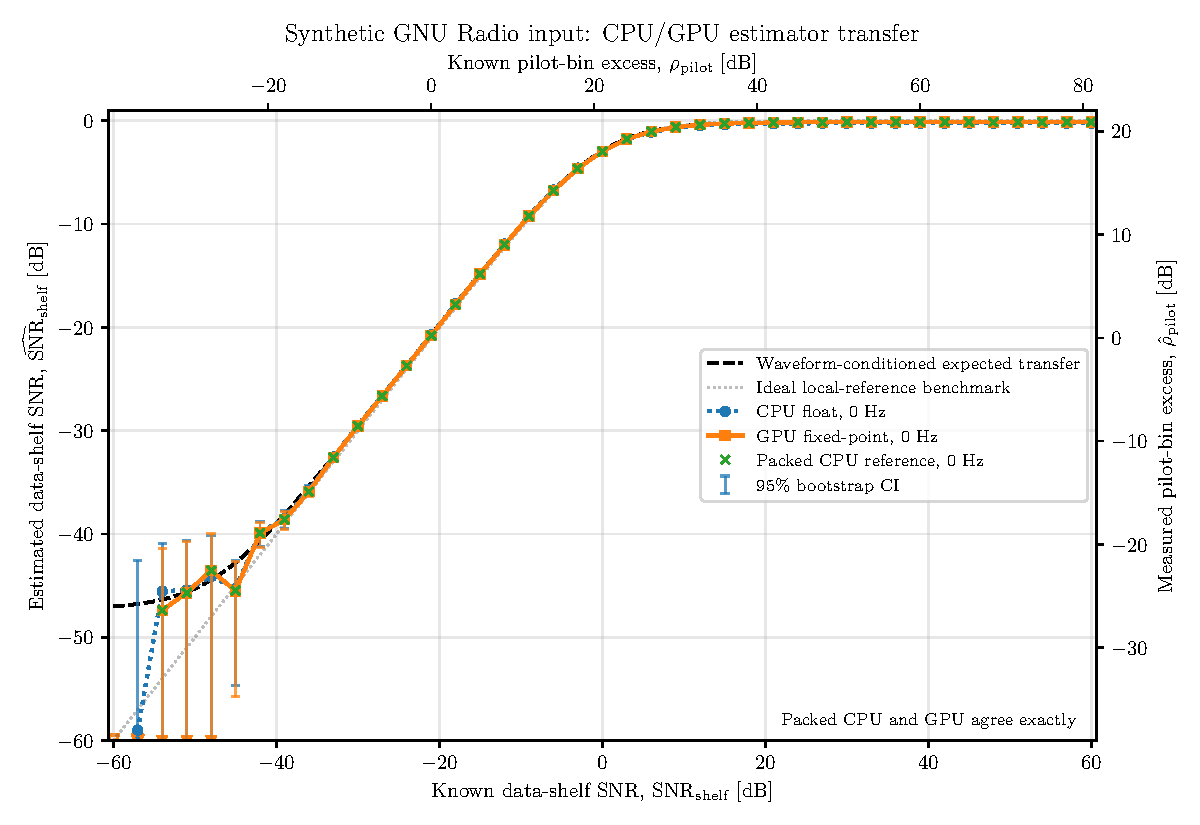
\includegraphics[width=0.98\linewidth]{figs/fig_estimator_transfer_digital.pdf}
\caption[Digital pilot-proxy estimator transfer]{Fully digital estimator transfer for a standards-chain 8-VSB waveform over data-shelf SNR from $-60$ to $+60$~dB in $3$~dB increments. Points show the floating-point CPU path, packed-integer CPU reference, and fixed-point GPU path; intervals are trial-bootstrap 95\% intervals. The ideal local-reference benchmark and the waveform-conditioned expectation are shown separately. The floating-point CPU central estimate is absent at $-60$~dB, while the packed CPU and GPU central estimates are absent at $-60$ and $-57$~dB. At those points the pooled normalized pilot excess is nonpositive, so its logarithm has no finite decibel value. These omissions mark the statistical estimator floor, not exhaustion of the fixed-point range. No threshold is applied. (The secondary axes label the pilot-bin excess $\rho_{\rm pilot}$; in the text that quantity is $e_p$ of Eq.~\eqref{eq:estimator:pilot-excess}, and $\rho$ is reserved for the CFAR rank.)}
\label{fig:estimator:digital-transfer}
\end{figure}

\subsection*{Controlled radio bridge}

The second experiment retains the estimator but adds minimal controlled over-the-air coupling. One LimeSDR \cite{limesdr} transmits and receives through its two antenna ports, separated by $1.45$~cm, at $485$~MHz with a $10.762$~MHz sample rate, $38$~dB transmit gain, and $8$~dB receive gain. Thirty randomized passes contain $1800$ mixture trials at commanded data-shelf SNRs from $-42$ to $0$~dB in $3$~dB increments. Each pass also contains transmitter-zero, signal-only, and noise-only controls; those controls calibrate the received input axis and the expected estimator response without treating the command value as the received SNR\@. They place the pooled received points from $-43.272$ to $-1.845$~dB.

\begin{figure}[H]
\centering
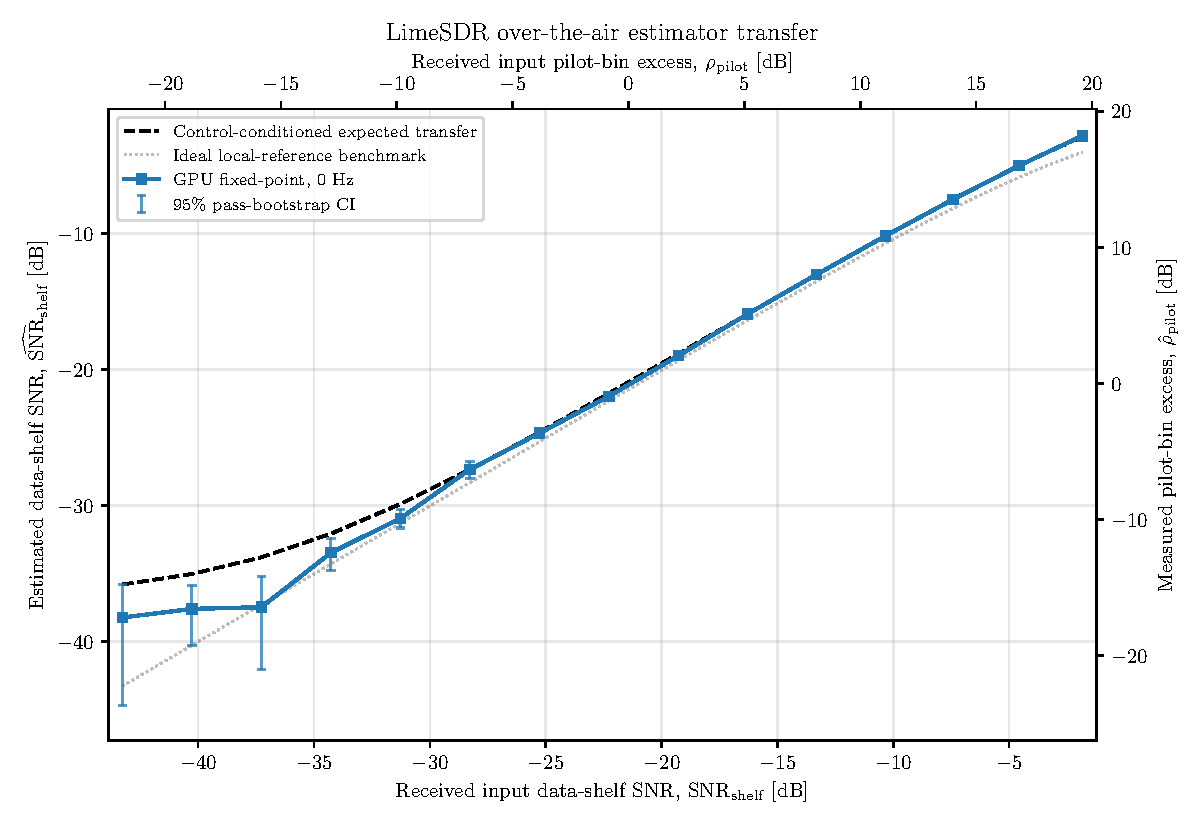
\includegraphics[width=0.98\linewidth]{figs/fig_ota_estimator_transfer.pdf}
\caption[Controlled over-the-air pilot-proxy estimator transfer]{Controlled LimeSDR over-the-air estimator transfer. The horizontal axis is received data-shelf SNR calibrated within each pass from transmitter-zero, signal-only, and noise-only controls; it is not the commanded transmit value. Points are fixed-point GPU estimates and intervals are 95\% pass-cluster bootstrap intervals, so a pass rather than an individual frame is the independent resampling unit. The control-conditioned expectation carries the same measured radio path and quantizer. This short two-port experiment is an estimator-transfer check, not a field-propagation, multipath-performance, or telescope-deployment study.}
\label{fig:estimator:ota-transfer}
\end{figure}

For commands from $-27$ to $0$~dB, corresponding to received inputs from $-28.273$ to $-1.845$~dB, fitting the measured output against the control-conditioned expected transfer gives slope approximately $1.0045$, intercept $0.026$~dB, and $R^2=0.99993$. The slope's 95\% pass-cluster interval is $[0.9917,1.0189]$ and the intercept interval is $[-0.101,0.168]$~dB. Direct measured-minus-control differences have RMS $0.084$~dB and maximum magnitude $0.208$~dB; residuals about the fitted line have RMS $0.065$~dB and maximum magnitude $0.137$~dB. The lower five command points expose the estimator floor near $-38$~dB rather than belonging to that linear fit. The experiment did not reach an upper estimator ceiling.

\stub{synthetic estimation rerun}{Repeat both sweeps at the production protocol and add the $g$ reconciliation of Section~\ref{sec:estimator:translation}: the waveform's spectral density at the reference bins relative to its flat top, the clean-waveform target-to-reference ratio, and the fitted saturation level, with the nominal value $1/2$ and the recorded $\approx 1$ both shown; replace Figures~\ref{fig:estimator:digital-transfer} and~\ref{fig:estimator:ota-transfer} and the fit coefficients quoted in the text.}

These experiments validate the \emph{estimation} stage represented by the coarse ratio and its model-based shelf-SNR inversion for the generated waveform and the control-conditioned radio setup. They do not establish a universal received pilot-to-allocation transfer, set or test a decision threshold, or measure $P_{\rm fa}$, $P_{\rm d}$, a receiver-operating curve, or a contamination-residual tolerance. They also do not substitute for a current-geometry study of the fine designated-set statistic with all $2048$ inputs and offset hypotheses. Those are detection questions carried into Chapter~\ref{sec:detection}; the controlled radio path is likewise not evidence of live telescope deployment.

\clearpage

\section{Offline Archive Estimation}
\label{sec:estimator:archive}

The archive processing surface evaluates the estimators of this chapter on CHIME's triggered full-array baseband captures. For every processed frame it retains the exact coarse integer power terms and the three exact integer fine-power spectra, so every statistic in this chapter can be recomputed from the product without any gain or loss assumption and independently of whatever mask the survey applied. Chapter~\ref{sec:survey} defines the capture inventory, validity rules, and product contract; Chapter~\ref{sec:calibration} then uses the retained estimators to identify each channel's current era and to measure its pilot anchor, null population, and sensitivity floor. This establishes that the estimator has been exercised on archive data under a pinned product contract. It does not make a retrospective archive mask a validated future operating threshold, and it does not make the triggered archive a sample of continuous observing time.

The observed null is the first test of the transfer. Under the idealized model of Section~\ref{sec:estimator:statistics} the normalized ratio $F/\mu_0$ is centred within a fraction of a percent of unity with a $0.24\%$ coarse width; the archive null is measured per channel on its current era, and the comparison has two parts: the centre, which tests the packed-weight prediction $\mu_0$, and the width, which measures how far receiver systematics inflate the i.i.d.\ model. In the superseded products the centre agreed with the packed-weight prediction to within \rerun{$0.13$~dB} on most channels with a usable null (to \rerun{$0.002$~dB} on channel 29), the channels that sat \rerun{$0.2$--$0.95$~dB} high were those with persistent occupancy, and the coarse width ran \rerun{$1.4$--$2.3\times$} the idealized prediction where the null was not visibly lifted. Reference-cell contamination can depress the ratio as well as target-cell contamination can raise it, so both sides of the empirical null require health checks.
\stub{v5 archive rerun}{Replace the previous sentence with the current-era null centres and widths from Table~\ref{tab:calibration:nulls}: per channel, the measured $F/\mu_0$ centre against $\mu_0$, the coarse and fine width factors against the i.i.d.\ model, and the fraction of channels within $0.1$~dB of prediction.}

The final offline protocol partitions each channel's current era by whole acquisition or contiguous time block. Calibration blocks freeze the validity rules, era definition, packed-weight null, estimator-floor treatment, and every pilot-to-shelf assumption. Those unchanged objects are then applied once to disjoint evaluation blocks. The evaluation reports the finite-estimate rate, pilot-inferred shelf-SNR distribution, null coverage, drift, repeatability, and block-bootstrap uncertainty. Frames from one acquisition are never divided randomly across both sides. The archive cannot measure absolute SNR error, because it contains neither a known injected SNR nor simultaneous truth across the full 6-MHz allocation; what it can measure is whether frozen calibration quantities transfer to untouched blocks.
\stub{v5 archive rerun}{Blocked-evaluation table: per channel, calibration-block and evaluation-block null centre and width, drift between blocks, finite-estimate rate, and block-bootstrap intervals.}

\section{Kotekan Stage and Live Estimation on the CHORD Pathfinder}
\label{sec:estimator:runtime}

The \texttt{kotekan} stage computes the same projection, coarse marginal, and fine path on the CHORD Pathfinder's voltage ring before visibility integration, using the Pathfinder profile of Section~\ref{sec:dtv:scope}: $K = 64$ over $N = 8192$ samples at $f_s = 195.3125$~kHz, which is $L = 128$ windows and the same $41.94$~ms frame, aligned one-to-one with the configured visibility integration. It binds physical channels through a runtime bundle, shares its estimator arithmetic with the archive path rather than redefining it for live use, and passes the file-based replay verifier of Chapter~\ref{sec:deployment}: dumped packed voltages replayed through the stage reproduce the metadata, bundle, packer, coarse powers, and mask bit-for-bit against the offline reference. The coarse marginal remains valuable as a low-cost diagnostic and exact verification tripwire even where it does not supply the decision.

The live estimation test is a predeclared multi-hour shadow run with one frozen channel bundle per monitored allocation. The stage records per-frame power terms, $F/\mu_0$, pilot-inferred shelf SNR, undefined estimates, health and tripwire state, bundle identity, runtime quantiles, and dropped or late frames. Sampled live frames are replayed through the independent offline reference, and stability is summarized by time block and channel. During this run the outputs do not alter visibility data. This test establishes live framing, continuous-stream stability, exact replay, and compute headroom; it does not establish absolute SNR accuracy without an independent received-shelf reference, and because the Pathfinder is a different receiver in a different transmitter environment, its null centres and widths are Pathfinder calibration data, not CHIME's.
\stub{Pathfinder shadow run}{Live estimation summary: run duration and frame count per channel; fraction of frames with finite estimates; time-block stability of $F/\mu_0$ and inferred shelf SNR; exact-replay agreement count on sampled frames; dropped and late frames; kernel and stage runtime quantiles.}

Chapter~\ref{sec:detection} supplies the separate policy layer that turns the estimator outputs into a calibrated rejection bit.
